\subsection{Results and conclusions}\label{sec:pbf_iterbin:conclusions}

I tested the three approaches on 12 samples from 4 different bacteria read samples, assembled by Unicycler, and where the contigs of size less than 100 were replaced by links in the assembly graph.
This subset covers several scenarios:

\begin{itemize}
  \item Some instances have connected components with only one contig looping on itself --- corresponding to circular plasmids (with, or without seeds);
  \item Some plasmids correspond to subgraph where a circular topology can be found (with or without seeds);
  \item Some plasmids correspond to subgraph where it is not possible to find a circular topology (missing links, with or without seeds).
\end{itemize}

\begin{warningbox}
  The Unicycler assembly graphs were malformed: some of the link definition were reversed (not in the sense of the reverse symmetry equivalence of defining one link and its reverse).
  This created many tips in the graph and denatured the cyclicity of subgraph corresponding to circular plasmids.
  However, many observations remain correct.
\end{warningbox}

\paragraph{The iterative binning process over-optimizes the first bin scores}
The first bin was mainly often the most difficult one to obtain.
In any case, the first bin is the largest one.
Each approach in the iterative binning process over-optimizes the scores of the first bin.
One of the main consequence is the first bin contains too much contigs, leading to remove contigs needed to get the next plasmids.
Thus, the next remain of plasmids are dispatched in several bins.
\Cref{fig:pbf_iterbin:merge_trap} provides a simple instance for which the iterative approach over-optimizes the first bin by merging several plasmids.
It also shows that additional bin topological constraint on the circularity does not solve the problem in the context of iterative binning.

\begin{figure}
  \centering
  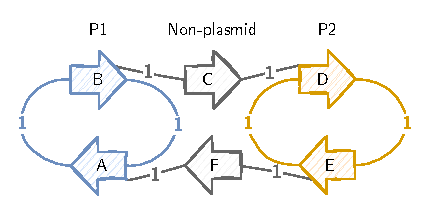
\includegraphics{pbf_iterbin/img/pbf_iterbin-merge_trap.pdf}
  \figurecaption{The first bin is more likely to be a merge of several plasmids.}{%
    Fragments of plasmid \(\mathsf{P1}\) (\(\mathsf{A}\) and \(\mathsf{B}\)) and those of plasmid \(\mathsf{P2}\) (\(\mathsf{D}\) and \(\mathsf{E}\)) are connected through two non-plasmid fragments (\(\mathsf{C}\) and \(\mathsf{F}\)).
    The number on links are their capacity in the network graph.
    As instance, let assume that the coverages of all the fragments equal \(1\), all the lengths equal \(100\), the plasmidness to be perfect (i.e.\ equal to \(1\) for plasmids' fragments and \(0\) for the others) as well as the seed set (containing only plasmids' fragments).
    Also, we consider only one GC content interval such that all the GC scores equal \(1\).
    The best bin is a merge of plasmid \(\mathsf{P1}\) and \(\mathsf{P2}\), corresponding to the flow \(\mathsf{S} \to \mathsf{A_f} \to \mathsf{B_f} \to \mathsf{C_f} \to \mathsf{D_f} \to \mathsf{E_f} \to \mathsf{T}\) (with score in \Cref{pbf_iterbin:once:mgclb:obj:max_coverage_score} equals to \(900\), for a total flow of \(1\)).
    Unfortunately, forcing the model to find a flow which can correspond to a circuit (circular bin) does not solve the problem here (the best bin remains a merge of \(\mathsf{P1}\) and \(\mathsf{P2}\), containing all the fragments).
  }\label{fig:pbf_iterbin:merge_trap}
\end{figure}

\paragraph{The MILP solving time is too long for a poor quality}
As described above, finding the first bin is the most difficult one to obtain, especially about time performance.
The MIP gap is sometimes really near to 0\% (optimal criterion) but slightly decreases.
Finding a MIP gap threshold for which we accept the feasible solution is not as easy, and no satisfying threshold was found (no more than 5\%).

\paragraph{Linearly handling the GC content of each contig seems to not be relevant}
Involving the GC content for plasmid binning through different non-intersecting intervals does not seem to help.
Here, we combine linearly the GC content of each contig through a positive flow passes.
While the flow can describe walks, we are not able (MILP limitation) to update the GC content of the extended sequence, and thus getting the true GC score for a given interval.
Note that GplasCC is updating the plasmid statistics each time it extends a walk (reconsider the whole extended sequence).

\paragraph{Connecting the source only to the seeds can split plasmid into several bins}
All the three approaches are based on a network graph where the source only connects the seeds.
When a link miss to satisfy the plasmid circularity, the recall and the precision become highly sensitive to the position of the seeds in the plasmid corresponding subgraph walk.
\Cref{fig:pbf_iterbin:seed_position_robustness} illustrates this issue.
As in \Cref{subfig:pbf_iterbin:middle_seed_splits_partially_circular_plasmid}, the recall decrease because we miss a fragment before the seed in the walk.
If this (positive plasmidness) fragment can be reached from another seed of another plasmid, it can appear in a different and wrong bin because it will enable to improve the objective function value at the time of this future bin search, resulting in a loss of precision.

\begin{figure}
  \centering
  \begin{subfigure}{0.45\linewidth}
    \centering
    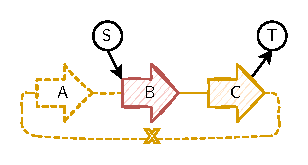
\includegraphics[width=\linewidth]{pbf_iterbin/img/pbf_iterbin-middle_seed_splits_partially_circular_plasmid.pdf}
    \caption{Seed splitting a partially circular bin}\label{subfig:pbf_iterbin:middle_seed_splits_partially_circular_plasmid}
  \end{subfigure}
  \hfill
  \begin{subfigure}{0.45\linewidth}
    \centering
    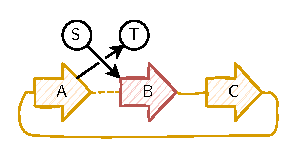
\includegraphics[width=\linewidth]{pbf_iterbin/img/pbf_iterbin-true_circularity_seed_robust.pdf}
    \caption{The circularity can avoid missing a fragment}\label{subfig:pbf_iterbin:true_circularity_seed_robust}
  \end{subfigure}
  \hfill
  \begin{subfigure}{\linewidth}
    \centering
    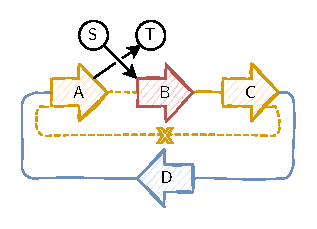
\includegraphics[width=0.45\linewidth]{pbf_iterbin/img/pbf_iterbin-circularity_artefact.pdf}
    \caption{A circularity artefact}\label{subfig:pbf_iterbin:circularity_artefact}
  \end{subfigure}
  \figurecaption{The search for a bin is highly sensitive to the seed position in a partially circular plasmid context}{%
    In each subfigure, fragments \(\mathsf{A}\), \(\mathsf{B}\) and \(\mathsf{C}\) and their links belong to the same plasmid.
    For all this fragments, we assume to be in an almost-perfect case: they all have the same coverage and the same best GC interval, and the plasmidness equals.
    However, the seed set only contains the red fragment \(\mathsf{B}\).
    A cross means the link does not exist while it should to satisfy the circularity of the plasmid.
    A dashed fragment or link is not active.
    %
    \Subref{subfig:pbf_iterbin:middle_seed_splits_partially_circular_plasmid}
    %
    The crossed link is missing so that it is not possible to complete the plasmid circularity.
    Since the seed is now in the middle of the path, and as according to the network definition the source only connects to the seed fragments, then the best bin misses the fragment \(\mathsf{A}\).
    %
    \Subref{subfig:pbf_iterbin:true_circularity_seed_robust}
    %
    If now the link is not missing, it is possible to retrieve \(\mathsf{A}\) by positioning it at the end of the walk, and outgoing after it to the sink (which connects to all the fragments).
    %
    \Subref{subfig:pbf_iterbin:circularity_artefact}
    %
    Suppose now we face the same situation as in \subref{subfig:pbf_iterbin:middle_seed_splits_partially_circular_plasmid} but fragment \(\mathsf{D}\) enables the circularity and is a fragment that does not belong to the orange plasmid.
    Under some circumstances, passing through this fragment can improve the objective function value because it enables to retrieve \(\mathsf{A}\).
    If \(b \in K\) is the GC content interval associated with the orange plasmid, then it is sufficient to have \( inflow(\mathsf{D}) (1 + \plm{\mathsf{D}} + \gcscore{\mathsf{D}}{b}) - \cov{\mathsf{D}} \geq 0\) to retrieve \(\mathsf{A}\) through \(\mathsf{D}\).

  }\label{fig:pbf_iterbin:seed_position_robustness}
\end{figure}

\paragraph{The positive flow constraint raises the complexity in a circular plasmid context}

As in PlasBin-flow, we require the flow on each arc to be at least equal to the total flow (i.e.\ the sum of the flow outgoing from the source).
The total flow thus conveniently encodes the multiplicity of a unique region in the genome the bin represents.
However, it increases the number of equivalent solutions in a circular plasmid context.
\Cref{fig:pbf_iterbin:implicit_circularity} illustrates this phenomenon.
Removing this constraint can improve the performances.
Also, it is the occasion to better model the circularity.

\begin{figure}
  \centering
  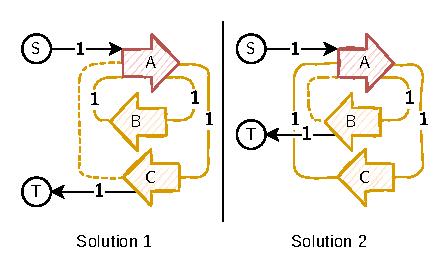
\includegraphics{pbf_iterbin/img/pbf_iterbin-implicit_circularity.pdf}
  \figurecaption{A repeated seed can split a bin}{%
    Suppose we have a plasmid with three fragments, where \(\mathsf{A}\) is the seed and also a repeated sequence in the plasmid genome, such that its coverage is twice the ones of \(\mathsf{B}\) and \(\mathsf{C}\).
    Dashed links are not active.
    Active links are associated with a flow number.
    Because we force the flow on the arcs to equal at least the total flow, in a circular context the best solutions consist in replacing one of the link that connects a unique region by the source-link and the sink-link, which emulate the circularity.
    This results in a set of equivalent solutions, and then to an increase of the branch-and-bound time consumption.
  }\label{fig:pbf_iterbin:implicit_circularity}
\end{figure}